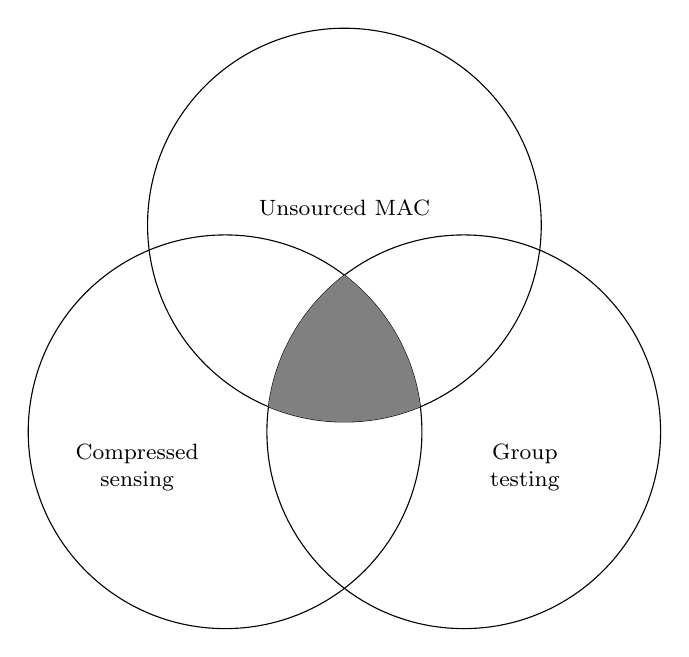
\begin{tikzpicture}
\def\fsize{\footnotesize}

	\def \r{2.5cm}
	\def\firstcircle{(90:1.75cm) circle (\r)}
  	\def\secondcircle{(210:1.75cm) circle (\r)}
	 \def\thirdcircle{(330:1.75cm) circle (\r)}
  
     \draw \firstcircle node[text=black,anchor=south] {\fsize{Unsourced MAC}};
    \draw \secondcircle node[text=black,anchor=north east] { %\fsize{Compressed sesning}};
    \fsize{\begin{tabular}{c}
    Compressed \\
    sensing\\
    \end{tabular}}
    };
    \draw \thirdcircle node[text=black,anchor=north west] {
        \fsize{\begin{tabular}{c}
	Group\\ testing\\ 
  \end{tabular}}
};
  
   \begin{scope}
    \clip \firstcircle;
    \clip \secondcircle;
    \fill[gray] \thirdcircle;
      \end{scope}

  \end{tikzpicture}